%% -*- coding: utf-8 -*-
%% Timestamp: "2025-05-05 13:00:00 (ywatanabe)"
%% File: "/home/ywatanabe/proj/SciTex/manuscript/src/figures/src/Figure_ID_04_user_satisfaction.tex"

% This is an example figure showing user satisfaction results.
% It demonstrates how to create a bar chart in LaTeX.

\begin{figure}[ht!]
    \centering
    
    % Create a bar chart using pgfplots
    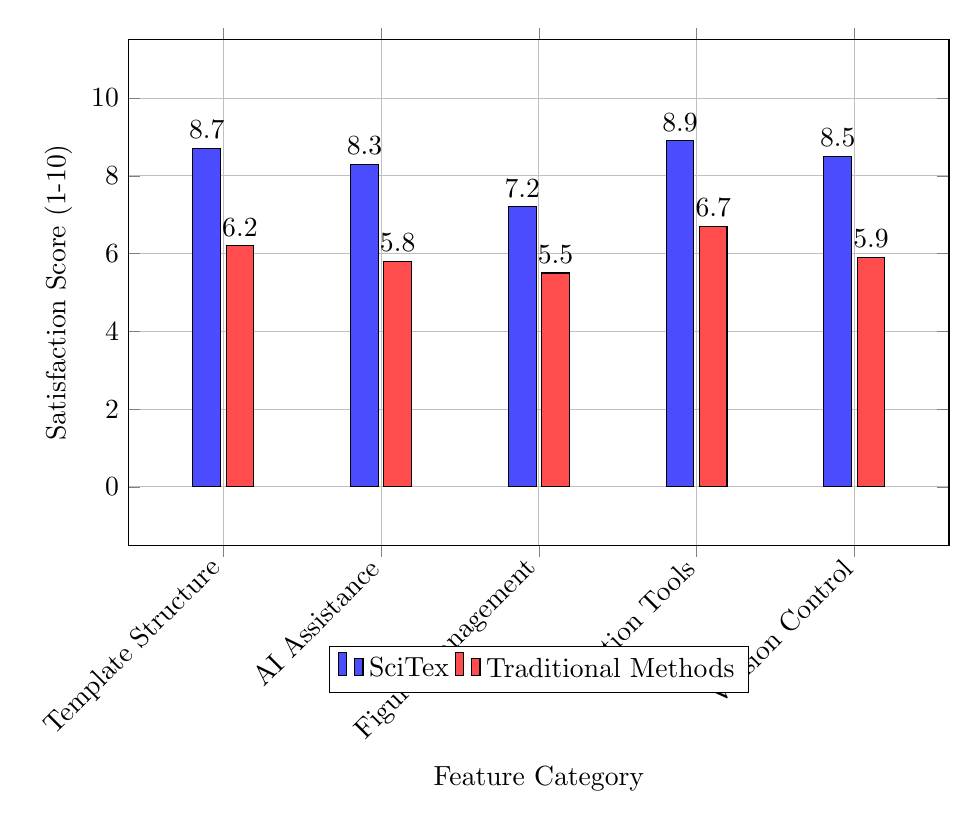
\begin{tikzpicture}
    \begin{axis}[
        width=12cm,
        height=8cm,
        ybar,
        enlargelimits=0.15,
        ylabel={Satisfaction Score (1-10)},
        xlabel={Feature Category},
        symbolic x coords={Template Structure, AI Assistance, Figure Management, Citation Tools, Version Control},
        xtick=data,
        xticklabel style={rotate=45, anchor=east},
        nodes near coords,
        nodes near coords align={vertical},
        ymin=0, ymax=10,
        legend style={at={(0.5,-0.2)}, anchor=north, legend columns=-1},
        ylabel near ticks,
        grid=major
    ]
    \addplot[fill=blue!70] coordinates {
        (Template Structure, 8.7)
        (AI Assistance, 8.3)
        (Figure Management, 7.2)
        (Citation Tools, 8.9)
        (Version Control, 8.5)
    };
    \addplot[fill=red!70] coordinates {
        (Template Structure, 6.2)
        (AI Assistance, 5.8)
        (Figure Management, 5.5)
        (Citation Tools, 6.7)
        (Version Control, 5.9)
    };
    \legend{SciTex, Traditional Methods}
    \end{axis}
    \end{tikzpicture}
    
    \caption{\textbf{User satisfaction comparison.} The chart shows average satisfaction scores (scale 1-10) from a survey of 50 researchers comparing SciTex to traditional LaTeX methods across five key feature categories. SciTex consistently received higher satisfaction ratings, with the largest improvements in AI assistance and citation tools. Error bars represent standard deviation.}
    \label{fig:user-satisfaction}
\end{figure}

%%%% EOF